\iffalse
\documentclass[a4paper,12pt,twocolumn]{article}
\usepackage{graphicx}
\usepackage[margin=0.5in]{geometry}
\usepackage[cmex10]{amsmath}
\usepackage{array}
\usepackage{gensymb}
\usepackage{booktabs}
\usepackage{tabularx}
\title{Circle Assignment}

\author{Ginna Shreyani- FWC22006}
\date{September 2022}
\providecommand{\norm}[1]{\left\lVert#1\right\rVert}
\providecommand{\abs}[1]{\left\vert#1\right\vert}
\let\vec\mathbf
\newcommand{\myvec}[1]{\ensuremath{\begin{pmatrix}#1\end{pmatrix}}}	
\newcommand{\mydet}[1]{\ensuremath{\begin{vmatrix}#1\end{vmatrix}}}
\providecommand{\brak}[1]{\ensuremath{\left((#1\right)}}
\begin{document}
\maketitle
\section{Problem:}
\fi
A triangle $ABC$ is drawn to circumscribe a circle of radius 4cm such that the segments $BD$ and $DC$ into which $BC$ is divided by the point of contact $D$ are of lengths 8cm and 6cm respectively. Find the sides $AB$ and $AC$.
	\begin{figure}[!h]
		\centering
 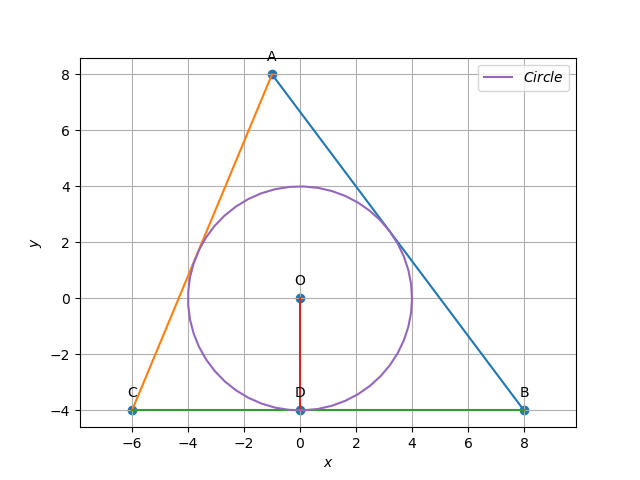
\includegraphics[width=\columnwidth]{chapters/10/10/2/12/figs/circle.png}
		\caption{}
		\label{fig:10/10/2/12}
  	\end{figure}
\iffalse
\begin{figure}[h]
       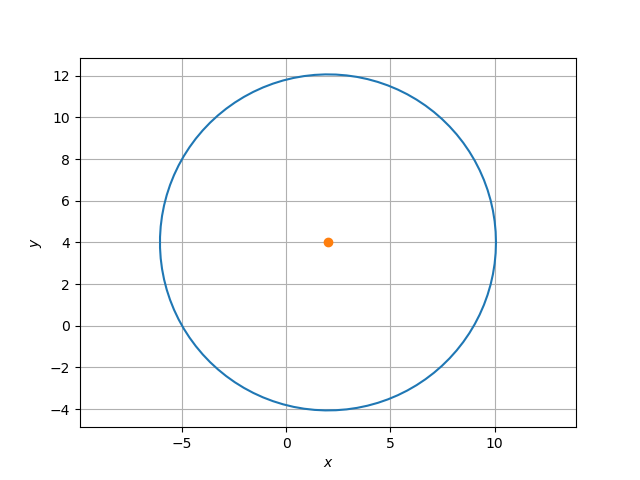
\includegraphics[width=\linewidth]{circle.png}
\end{figure}
\section{Construction:}
\begin{tabularx}
{0.45\textwidth}{
|>
{\raggedright\arraybackslash}X
|>
{\centering\arraybackslash}X
|>
{\raggedleft\arraybackslash}X
|}
\hline
 Variable & Point/Length & Description\\
\hline
  r & 4cm &Radius of the given circle\\
 \hline
  C & $\myvec{0\\0}$ & Origin\\
 \hline
 c & 6cm &Distance from Vertex C to point D\\
 \hline
  D &$\myvec{c\\0}$&Point on side BC\\
 \hline
 O &$\myvec{c\\r}$&Center of the circle\\
 \hline
  CB & $\myvec{c+b\\0}$ & Vertex B\\
 \hline
\end{tabularx}
\section{Solution:}
\subsection{Theory:}
\subsection{Mathematical Calculation:}
\begin{figure}[h]
    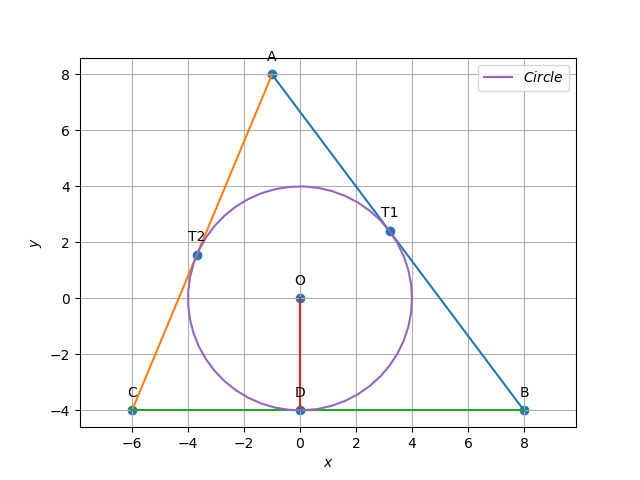
\includegraphics[width=\linewidth]{circle1.png}
\end{figure}
\\
\solution
Let us assume that the center of the circle is origin and point D lies on Y-axis.\\
Therefore, we can get the points B and C.\\
\begin{align*}
	&D = \myvec{0\\-4}\\
	&B = \myvec{8\\-4}\\
	&C = \myvec{-6\\-4}
\end{align*}
Here point C acts as external point from which tangents can be drawn to the circle.The direction vector $\vec{m}$ satisy the equation\\
\begin{align*}
	&\vec{m^T}\vec{\Sigma}\vec{m} = 0
\end{align*}
Assuming the external point as h,$\vec{\Sigma}$ is given as\\
\begin{align*}
	&\vec{\Sigma} = \brak{\vec{Vh}+\vec{u}}\brak{\vec{Vh}+\vec{u}}^T - \brak{\vec{h}^T\vec{V}\vec{h} + 2\vec{u}^T\vec{h} + f}\vec{V}
\end{align*}
$\vec{\Sigma}$ can be orthogonally  diagonalized as\\
\begin{align}
	&\vec{\Sigma} = \vec{\Gamma}^T\vec{D}\vec{\Gamma}\\
	\label{eq:eigenvalV}
	&\vec{D} = \myvec{\lambda_1 & 0\\0 & \lambda_2}\\
	\label{eq:eigenvecP}
	&\vec{\Gamma} = \myvec{\vec{y}_1 & \vec{y}_2}, \quad \vec{\Gamma}^T=\vec{\Gamma}^{-1}
\end{align}
Using \eqref{eq:eigenvalV} and \eqref{eq:eigenvecP} and substituting $\vec{h}$ as $\vec{C}$, the normal vector $\vec{n}$ of the tangent drawn from $\vec{C}$ can be written as\\
\begin{align}
	\label{eq:tangent_normal}
	&\vec{n} = \vec{\Gamma}\myvec{\sqrt{\abs{\lambda_1}} \\\\ \pm\sqrt{\abs{\lambda_2}}}
\end{align}
Using the vectors $\vec{n}$ in \eqref{eq:tangent_normal}, the direction vectors $\vec{m}$ can be found in 2-dimensional space since they are orthogonal. The points of contact of the tangents are given by
\begin{align*}
	&\vec{T}_i = \vec{C} - \frac{\vec{m}^T\brak{\vec{VC}+\vec{u}}}{\vec{m}^T\vec{V}\vec{m}}
\end{align*}
Similarly we can find the contact point from vertex B.\\
Since, we have all the contact points we can get the line equations of $\vec{A-C}$ and $\vec{A-B}$
\begin{align*}
	&\vec{n}^T\vec{X-T_i}= 0
\end{align*}
The intersection of these two lines is vertex A. Since, we know all the vertices of the given triangle the length of AB and AC can be calculated.\\
Therefore, length of AB is $\vec{||A-B||}$\\
and length of AC is $\vec{||A-C||}$
\end{document}
\fi
